\documentclass[12pt,a4paper]{article}
\usepackage[utf8]{inputenc}
\usepackage[T1]{fontenc}
\usepackage{geometry}
\usepackage{amsmath, amssymb}
\usepackage{listings}
\usepackage{xcolor}
\usepackage{booktabs}
\usepackage{array}
\usepackage{hyperref}
\usepackage{tikz}
\usetikzlibrary{positioning, arrows.meta, matrix}

\geometry{left=2.5cm, right=2.5cm, top=2.5cm, bottom=2.5cm}

\definecolor{codebg}{rgb}{0.96,0.96,0.96}
\definecolor{codegreen}{rgb}{0.0,0.5,0.0}
\definecolor{codegray}{rgb}{0.5,0.5,0.5}
\definecolor{codepurple}{rgb}{0.58,0,0.82}
\definecolor{codeblue}{rgb}{0.0,0.0,0.8}
\definecolor{negativered}{rgb}{0.7,0.0,0.0}

\lstdefinestyle{javastyle}{
    backgroundcolor=\color{codebg},
    commentstyle=\color{codegreen}\itshape,
    keywordstyle=\color{codeblue}\bfseries,
    stringstyle=\color{codepurple},
    numberstyle=\tiny\color{codegray},
    basicstyle=\ttfamily\small,
    breaklines=true,
    keepspaces=true,
    numbers=left,
    numbersep=5pt,
    language=Java,
    frame=single,
    rulecolor=\color{codegray}
}

\hypersetup{colorlinks=true, linkcolor=blue, urlcolor=cyan}

\title{
    \Huge \textbf{Shortest Path Algorithms} \\[0.5em]
    \Large Dijkstra's $\cdot$ Bellman-Ford $\cdot$ Floyd-Warshall \\[0.5em]
    \large Data Structures \& Algorithms Reference
}
\author{Algorithm Study Guide}
\date{\today}

\begin{document}

\maketitle
\tableofcontents
\newpage

% ============================================================
\section{Introduction to Shortest Path Problems}
% ============================================================

\subsection{Problem Statement}
Given a weighted directed (or undirected) graph $G = (V, E, w)$, the \textbf{shortest path} from vertex $s$ to vertex $t$ is a path $p = \langle v_0, v_1, \ldots, v_k \rangle$ where $v_0 = s$, $v_k = t$, and the total weight:
\[
w(p) = \sum_{i=1}^{k} w(v_{i-1}, v_i)
\]
is minimized among all paths from $s$ to $t$.

\subsection{Variants}
\begin{itemize}
    \item \textbf{Single-Source Shortest Path (SSSP)}: Shortest paths from one source $s$ to all other vertices. (Dijkstra's, Bellman-Ford)
    \item \textbf{Single-Destination}: Shortest paths from all vertices to one destination.
    \item \textbf{All-Pairs Shortest Path (APSP)}: Shortest paths between every pair $(u,v)$. (Floyd-Warshall)
\end{itemize}

\subsection{Edge Relaxation}
The core operation in shortest path algorithms is \textbf{edge relaxation}:
\[
\text{if } d[u] + w(u,v) < d[v]:\quad d[v] \leftarrow d[u] + w(u,v)
\]
This updates the best known distance to $v$ if a shorter path through $u$ is found.

\subsection{Complexity Summary}
\begin{table}[h!]
\centering
\renewcommand{\arraystretch}{1.4}
\begin{tabular}{|l|c|c|c|c|}
\hline
\textbf{Algorithm}    & \textbf{Time}  & \textbf{Space} & \textbf{Negative Weights} & \textbf{Scope} \\
\hline
Dijkstra's (Heap)     & $O(E \log V)$  & $O(V)$         & No ($w \geq 0$ only)      & Single source  \\
Bellman-Ford          & $O(VE)$        & $O(V)$         & Yes + cycle detection     & Single source  \\
Floyd-Warshall        & $O(V^3)$       & $O(V^2)$       & Yes (no neg cycles)       & All pairs      \\
\hline
\end{tabular}
\caption{$V$ = vertices, $E$ = edges}
\end{table}

\newpage

% ============================================================
\section{Dijkstra's Algorithm}
% ============================================================

\subsection{Concept}
Dijkstra's is a \textbf{greedy algorithm} for SSSP. It maintains a set of vertices whose shortest distance from the source is finalized, and greedily expands to the nearest unfinalized vertex.

\textbf{Key idea}: At each step, pick the vertex $u$ with the minimum $d[u]$ and relax all its outgoing edges.

\subsection{Algorithm Steps}
\begin{enumerate}
    \item Initialize: $d[s] = 0$, $d[v] = \infty$ for all $v \ne s$.
    \item Insert all vertices into a \textbf{Min-Heap} with priority $d[v]$.
    \item While Min-Heap is not empty:
    \begin{enumerate}
        \item Extract vertex $u$ with minimum $d[u]$.
        \item For each neighbor $v$ of $u$:
        \[
        \text{if } d[u] + w(u,v) < d[v]:\quad d[v] \leftarrow d[u] + w(u,v)
        \]
        \item Update $v$ in Min-Heap.
    \end{enumerate}
\end{enumerate}

\subsection{Example}

\begin{center}
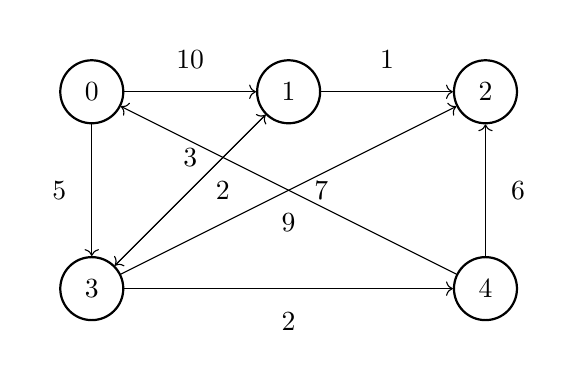
\begin{tikzpicture}[
    node distance=2.5cm,
    every node/.style={circle, draw, thick, minimum size=0.8cm},
    every edge/.style={draw, thick, ->}
]
\node (0) {0};
\node (1) [right of=0] {1};
\node (3) [below of=0] {3};
\node (2) [right of=1] {2};
\node (4) [below of=2] {4};

\draw[->] (0) -- node[above,draw=none]{10} (1);
\draw[->] (0) -- node[left,draw=none]{5}  (3);
\draw[->] (1) -- node[above,draw=none]{1} (2);
\draw[->] (1) -- node[right,draw=none]{2} (3);
\draw[->] (3) -- node[above,draw=none]{3} (1);
\draw[->] (3) -- node[below,draw=none]{9} (2);
\draw[->] (3) -- node[below,draw=none]{2} (4);
\draw[->] (4) -- node[right,draw=none]{6} (2);
\draw[->] (4) -- node[right,draw=none]{7} (0);
\end{tikzpicture}
\end{center}

\textbf{Shortest distances from vertex 0}: $d = [0, 8, 9, 5, 7]$

\subsection{Java Implementation}
\begin{lstlisting}[style=javastyle, caption={Dijkstra's Algorithm — Java}]
public static int[] dijkstra(List<List<Edge>> adjList, int V, int src) {
    int[] dist = new int[V];
    Arrays.fill(dist, Integer.MAX_VALUE / 2);
    dist[src] = 0;

    PriorityQueue<int[]> pq =
        new PriorityQueue<>(Comparator.comparingInt(a -> a[0]));
    pq.offer(new int[]{0, src});

    while (!pq.isEmpty()) {
        int[] curr = pq.poll();
        int u = curr[1];
        if (curr[0] > dist[u]) continue; // Stale entry

        for (Edge e : adjList.get(u)) {
            int newDist = dist[u] + e.weight;
            if (newDist < dist[e.dest]) {
                dist[e.dest] = newDist;
                pq.offer(new int[]{dist[e.dest], e.dest});
            }
        }
    }
    return dist;
}
\end{lstlisting}

\subsection{Complexity}
\begin{itemize}
    \item \textbf{Time}: $O(E \log V)$ with adjacency list + Min-Heap.
    \item \textbf{Space}: $O(V)$ for the distance array.
    \item \textbf{Limitation}: \textcolor{negativered}{\textbf{Does NOT work with negative edge weights!}} The greedy assumption breaks because a shorter path via a negative edge could be found later.
\end{itemize}

\subsection{Applications}
\begin{itemize}
    \item \textbf{GPS Navigation} (Google Maps, Waze).
    \item \textbf{Network routing} (OSPF protocol uses Dijkstra's).
    \item \textbf{Game AI} pathfinding (extended as A* with a heuristic).
    \item \textbf{Social networks}: finding shortest connection chains.
\end{itemize}

\newpage

% ============================================================
\section{Bellman-Ford Algorithm}
% ============================================================

\subsection{Concept}
Bellman-Ford is a \textbf{dynamic programming} approach for SSSP. It relaxes \textbf{all edges} $V-1$ times. After $k$ iterations, $d[v]$ holds the shortest path from $s$ to $v$ using at most $k$ edges. Since any shortest path (without negative cycles) uses at most $V-1$ edges, $V-1$ iterations suffice.

\subsection{Algorithm Steps}
\begin{enumerate}
    \item Initialize: $d[s] = 0$, $d[v] = \infty$ for all $v \ne s$.
    \item Repeat $V - 1$ times:
    \[
    \forall (u,v,w) \in E:\quad \text{if } d[u] + w < d[v],\;\text{set } d[v] = d[u] + w
    \]
    \item \textbf{Negative Cycle Detection} (one extra pass):
    \[
    \text{If any } d[v] \text{ can still decrease} \Rightarrow \text{negative cycle exists!}
    \]
\end{enumerate}

\subsection{Why $V - 1$ Iterations?}
In a graph with $V$ vertices, any simple path (no repeated vertices) has at most $V - 1$ edges. Each iteration of Bellman-Ford ``discovers'' paths with one more edge. After $V-1$ iterations, all shortest paths are known.

\subsection{Negative Cycle Detection}
A \textbf{negative cycle} is a cycle whose total edge weight is negative. If one exists, shortest paths are undefined (we can keep going around the cycle to decrease cost indefinitely).

Bellman-Ford detects this by checking: after $V-1$ relaxations, if any edge can still be relaxed, a negative cycle exists.

\subsection{Java Implementation}
\begin{lstlisting}[style=javastyle, caption={Bellman-Ford Algorithm — Java}]
public static void bellmanFord(int V, int[][] edges, int src) {
    int INF = Integer.MAX_VALUE / 2;
    int[] dist = new int[V];
    Arrays.fill(dist, INF);
    dist[src] = 0;

    // Relax all edges V-1 times
    for (int i = 1; i <= V - 1; i++) {
        for (int[] edge : edges) {
            int u = edge[0], v = edge[1], w = edge[2];
            if (dist[u] != INF && dist[u] + w < dist[v])
                dist[v] = dist[u] + w;
        }
    }

    // Detect negative cycle (V-th relaxation pass)
    for (int[] edge : edges) {
        int u = edge[0], v = edge[1], w = edge[2];
        if (dist[u] != INF && dist[u] + w < dist[v]) {
            System.out.println("Negative cycle detected!");
            return;
        }
    }
}
\end{lstlisting}

\subsection{Complexity}
\begin{itemize}
    \item \textbf{Time}: $O(VE)$ — $V-1$ passes, each iterating over $E$ edges.
    \item \textbf{Space}: $O(V)$ for the distance array.
    \item \textbf{Advantages over Dijkstra's}:
    \begin{itemize}
        \item Handles \textbf{negative edge weights}.
        \item \textbf{Detects negative cycles}.
    \end{itemize}
\end{itemize}

\subsection{Applications}
\begin{itemize}
    \item \textbf{Financial arbitrage detection} (negative cycle = profit loop in currency exchange).
    \item \textbf{Network routing} (Routing Information Protocol — RIP).
    \item \textbf{Distance vector protocols} in networking.
\end{itemize}

\newpage

% ============================================================
\section{Floyd-Warshall Algorithm}
% ============================================================

\subsection{Concept}
Floyd-Warshall is a \textbf{dynamic programming} algorithm for \textbf{All-Pairs Shortest Path (APSP)}. It computes the shortest path between every pair of vertices $(i, j)$ by considering each vertex $k$ as a potential intermediate node.

\subsection{Recurrence}
Let $d^{(k)}[i][j]$ = shortest path from $i$ to $j$ using only intermediate vertices from $\{0, 1, \ldots, k\}$:

\[
d^{(k)}[i][j] = \min\!\left(d^{(k-1)}[i][j],\;\; d^{(k-1)}[i][k] + d^{(k-1)}[k][j]\right)
\]

\textbf{Meaning}: The shortest path from $i$ to $j$ either:
\begin{itemize}
    \item Does \textbf{not} go through $k$: $d^{(k-1)}[i][j]$
    \item Goes \textbf{through} $k$: $d^{(k-1)}[i][k] + d^{(k-1)}[k][j]$
\end{itemize}

\subsection{Algorithm Steps}
\begin{enumerate}
    \item Initialize: $d[i][j] = w(i,j)$ if edge exists, $\infty$ otherwise, $d[i][i] = 0$.
    \item For $k = 0$ to $V-1$:
          \quad For all pairs $(i,j)$: relax via intermediate vertex $k$.
    \item Check: if $d[i][i] < 0$ for any $i$ $\Rightarrow$ negative cycle.
\end{enumerate}

\subsection{Example}

Initial matrix (INF = $\infty$):
\[
D = \begin{pmatrix} 0 & 3 & \infty & 7 \\ 8 & 0 & 2 & \infty \\ 5 & \infty & 0 & 1 \\ 2 & \infty & \infty & 0 \end{pmatrix}
\]

After Floyd-Warshall, $D[i][j]$ gives the shortest path from $i$ to $j$ for all pairs.

\subsection{Java Implementation}
\begin{lstlisting}[style=javastyle, caption={Floyd-Warshall Algorithm — Java}]
public static void floydWarshall(int[][] graph, int V) {
    int[][] dist = new int[V][V];
    for (int i = 0; i < V; i++)
        dist[i] = Arrays.copyOf(graph[i], V);

    for (int k = 0; k < V; k++) {
        for (int i = 0; i < V; i++) {
            for (int j = 0; j < V; j++) {
                if (dist[i][k] != INF && dist[k][j] != INF)
                    dist[i][j] = Math.min(dist[i][j],
                                          dist[i][k] + dist[k][j]);
            }
        }
    }

    // Negative cycle detection
    for (int i = 0; i < V; i++)
        if (dist[i][i] < 0) { System.out.println("Neg cycle!"); return; }
}
\end{lstlisting}

\subsection{Complexity}
\begin{itemize}
    \item \textbf{Time}: $O(V^3)$ — three nested loops over $V$ vertices.
    \item \textbf{Space}: $O(V^2)$ for the $V \times V$ distance matrix.
    \item \textbf{Limitation}: Expensive for large graphs ($V > 1000$ becomes slow).
\end{itemize}

\subsection{Applications}
\begin{itemize}
    \item \textbf{All-pairs shortest paths} in networks (e.g., routing tables).
    \item \textbf{Transitive closure} of a directed graph.
    \item \textbf{Network latency} between all pairs of servers.
    \item \textbf{Game pathfinding} when precomputing all pairwise distances.
\end{itemize}

\newpage

% ============================================================
\section{Comparison of All Three Algorithms}
% ============================================================

\begin{table}[h!]
\centering
\renewcommand{\arraystretch}{1.5}
\begin{tabular}{|l|p{3.5cm}|p{3.5cm}|p{3.5cm}|}
\hline
\textbf{Property}    & \textbf{Dijkstra's}       & \textbf{Bellman-Ford}       & \textbf{Floyd-Warshall}    \\
\hline
Approach             & Greedy                    & Dynamic Programming         & Dynamic Programming         \\
Scope                & Single source             & Single source               & All pairs                   \\
Time                 & $O(E \log V)$             & $O(VE)$                     & $O(V^3)$                    \\
Space                & $O(V)$                    & $O(V)$                      & $O(V^2)$                    \\
Negative Weights     & \textcolor{negativered}{No}    & \textcolor{codegreen}{Yes} & \textcolor{codegreen}{Yes} \\
Negative Cycle Detection & No                   & \textcolor{codegreen}{Yes}  & \textcolor{codegreen}{Yes} \\
Best For             & Large sparse graphs, non-negative weights & Graphs with negative edges & Small dense graphs, all-pairs \\
\hline
\end{tabular}
\caption{Shortest Path Algorithm Comparison}
\end{table}

\section{Key Formulas}

\begin{align}
\text{Edge Relaxation:}\quad         & d[v] = \min(d[v],\; d[u] + w(u,v)) \\[4pt]
\text{Dijkstra's:}\quad              & T = O(E \log V) \\[4pt]
\text{Bellman-Ford:}\quad            & T = O(VE),\quad \text{runs } V-1 \text{ passes} \\[4pt]
\text{Floyd-Warshall DP:}\quad       & d^{(k)}[i][j] = \min\!\left(d^{(k-1)}[i][j],\;d^{(k-1)}[i][k]+d^{(k-1)}[k][j]\right) \\[4pt]
\text{Floyd-Warshall:}\quad          & T = O(V^3),\quad S = O(V^2)
\end{align}

\end{document}
